\documentclass[tikz,border=3pt]{standalone}
\usepackage[T1]{fontenc}
\usepackage{lmodern}
\usetikzlibrary{arrows.meta,positioning,fit,backgrounds}
\definecolor{kubeblue}{HTML}{2E6F9E}
\definecolor{gateblue}{HTML}{D9EAF5}
\definecolor{softgray}{HTML}{F1F3F5}
\definecolor{evidencegreen}{HTML}{E3F1EA}
\begin{document}
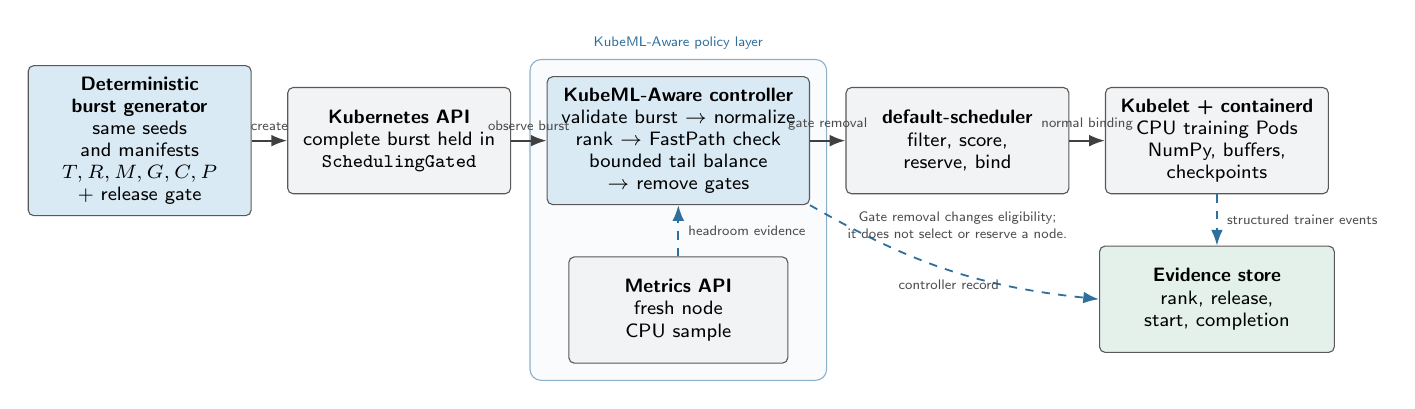
\begin{tikzpicture}[
  font=\sffamily\scriptsize,
  box/.style={draw=black!65, rounded corners=2pt, minimum height=1.35cm,
              text width=2.55cm, align=center, inner sep=4pt},
  main/.style={box, fill=gateblue},
  native/.style={box, fill=softgray},
  evidence/.style={box, fill=evidencegreen},
  flow/.style={-{Latex[length=2mm]}, line width=0.75pt, draw=black!75},
  feedback/.style={-{Latex[length=2mm]}, line width=0.65pt, draw=kubeblue, dashed},
  note/.style={font=\sffamily\tiny, align=center, text=black!70}
]

\node[main] (generator) {\textbf{Deterministic burst generator}\\
same seeds and manifests\\$T,R,M,G,C,P$ + release gate};

\node[native, right=0.45cm of generator] (api) {\textbf{Kubernetes API}\\
complete burst held in\\\texttt{SchedulingGated}};

\node[main, right=0.45cm of api, text width=3.05cm] (controller) {\textbf{KubeML-Aware controller}\\
validate burst $\rightarrow$ normalize\\rank $\rightarrow$ FastPath check\\bounded tail balance $\rightarrow$ remove gates};

\node[native, right=0.45cm of controller] (scheduler) {\textbf{default-scheduler}\\
filter, score, reserve, bind};

\node[native, right=0.45cm of scheduler] (node) {\textbf{Kubelet + containerd}\\
CPU training Pods\\NumPy, buffers, checkpoints};

\draw[flow] (generator) -- node[above,note]{create} (api);
\draw[flow] (api) -- node[above,note]{observe burst} (controller);
\draw[flow] (controller) -- node[above,note]{gate removal} (scheduler);
\draw[flow] (scheduler) -- node[above,note]{normal binding} (node);

\node[native, below=0.65cm of controller, text width=2.5cm] (metrics) {\textbf{Metrics API}\\fresh node CPU sample};
\draw[feedback] (metrics) -- node[right,note]{headroom evidence} (controller);

\node[evidence, below=0.65cm of node, text width=2.7cm] (store) {\textbf{Evidence store}\\rank, release, start, completion};
\draw[feedback] (controller.south east) to[bend right=12] node[below,note]{controller record} (store.west);
\draw[feedback] (node) -- node[right,note]{structured trainer events} (store);

\node[note, below=0.10cm of scheduler, text width=2.8cm] {Gate removal changes eligibility;\\it does not select or reserve a node.};

\begin{scope}[on background layer]
  \node[draw=kubeblue!55, rounded corners=4pt, fit=(controller)(metrics),
        inner sep=6pt, fill=kubeblue!3, label={[font=\sffamily\tiny,text=kubeblue]above:KubeML-Aware policy layer}] {};
\end{scope}

\end{tikzpicture}
\end{document}
